\section{Première analyse des données}

\textbf{Question 1: Visualisation des données en 2D et 3D}

\begin{figure}[!h]
    \begin{minted}[frame=lines, framesep=2mm, baselinestretch=1.2, fontsize=\footnotesize, linenos, breaklines=true]{python}
def preprocessing():
    # [...]
    displayFeatures2d(feat)
    displayFeatures3d(feat)

    return feat, img73, img87
    \end{minted}   
    \captionof{listing}{\label{lst:VisualisationFunction}Visualisation Function}
\end{figure}

\begin{figure}[!h]
    \begin{minipage}{.40\linewidth}
        \begin{center}
            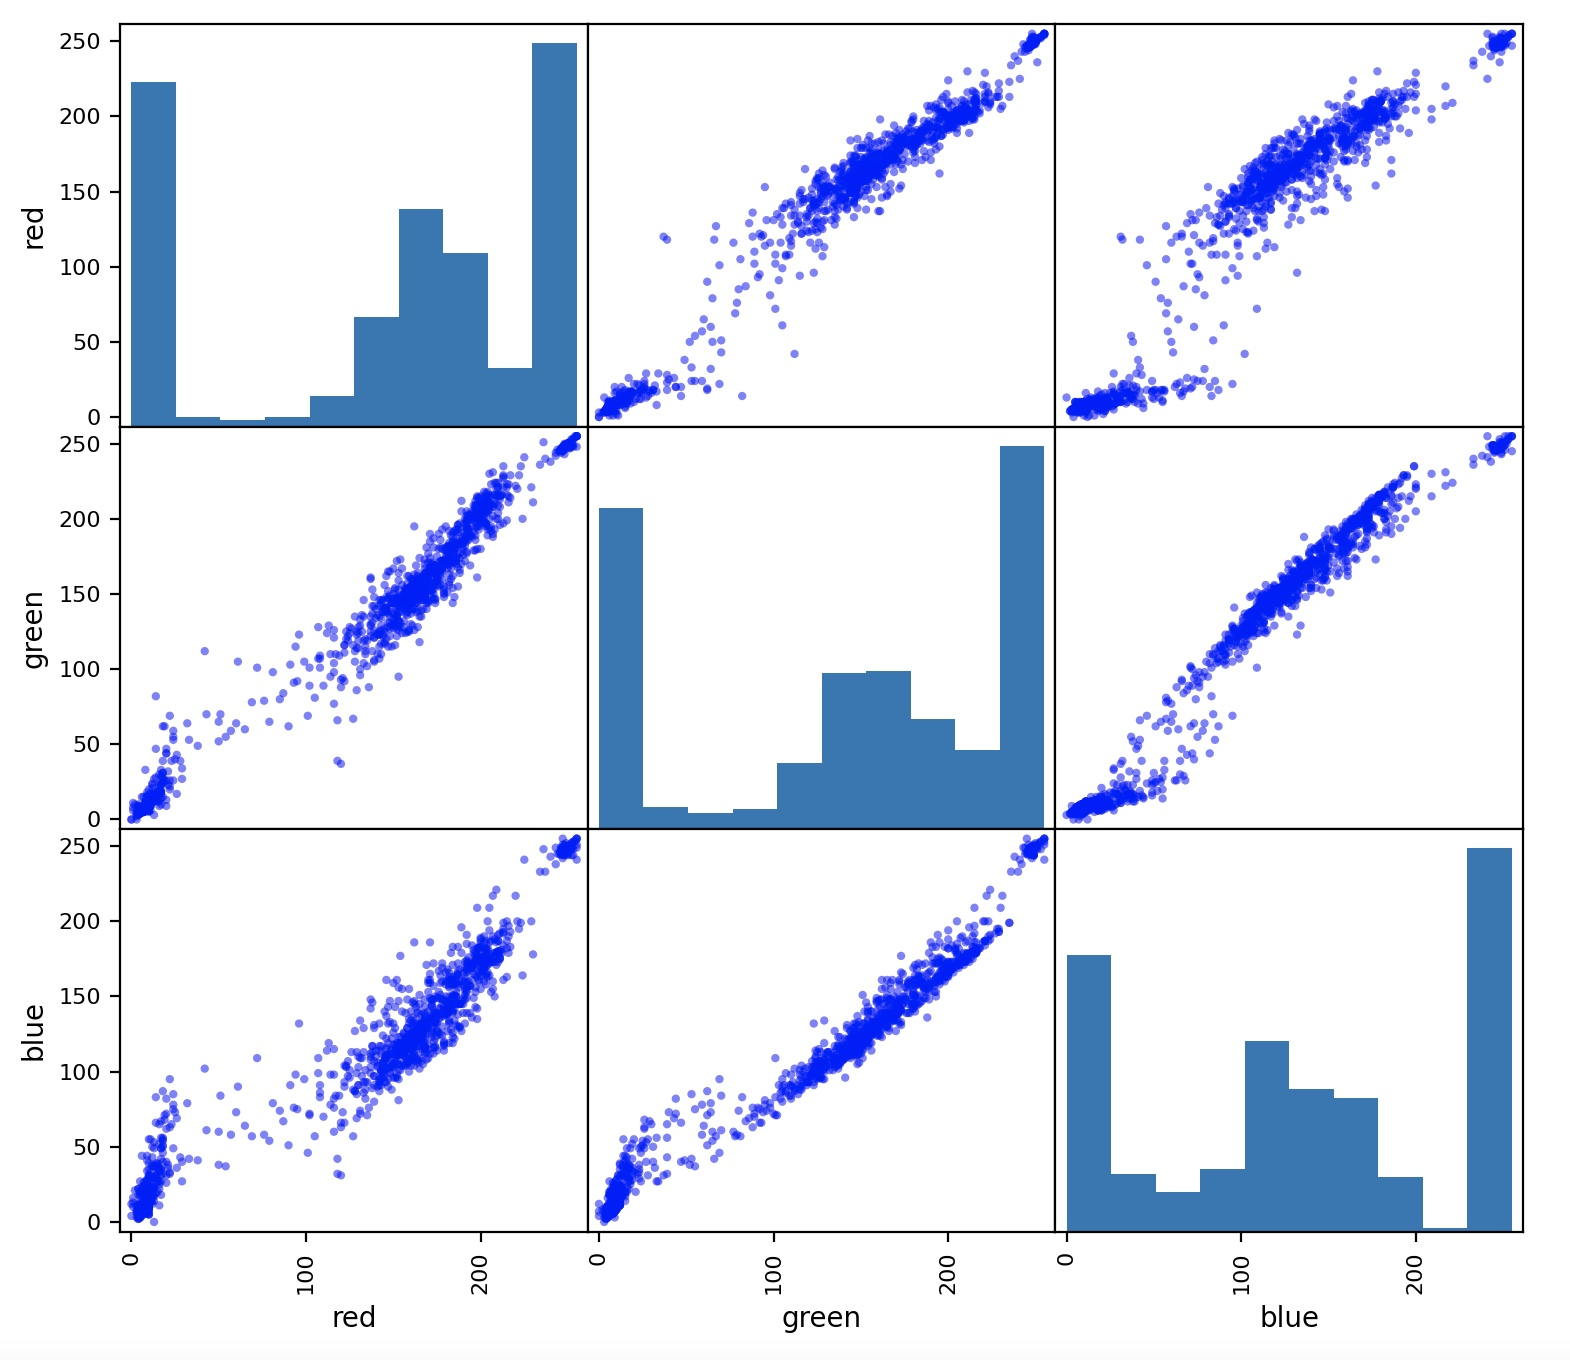
\includegraphics[width=0.75\textwidth]{./img/5.1.2.jpg}
                \caption{\label{fig:1.2}Image 2D}  
            \end{center}
    \end{minipage}\hfill
    \begin{minipage}{.56\linewidth}
        \begin{center}
            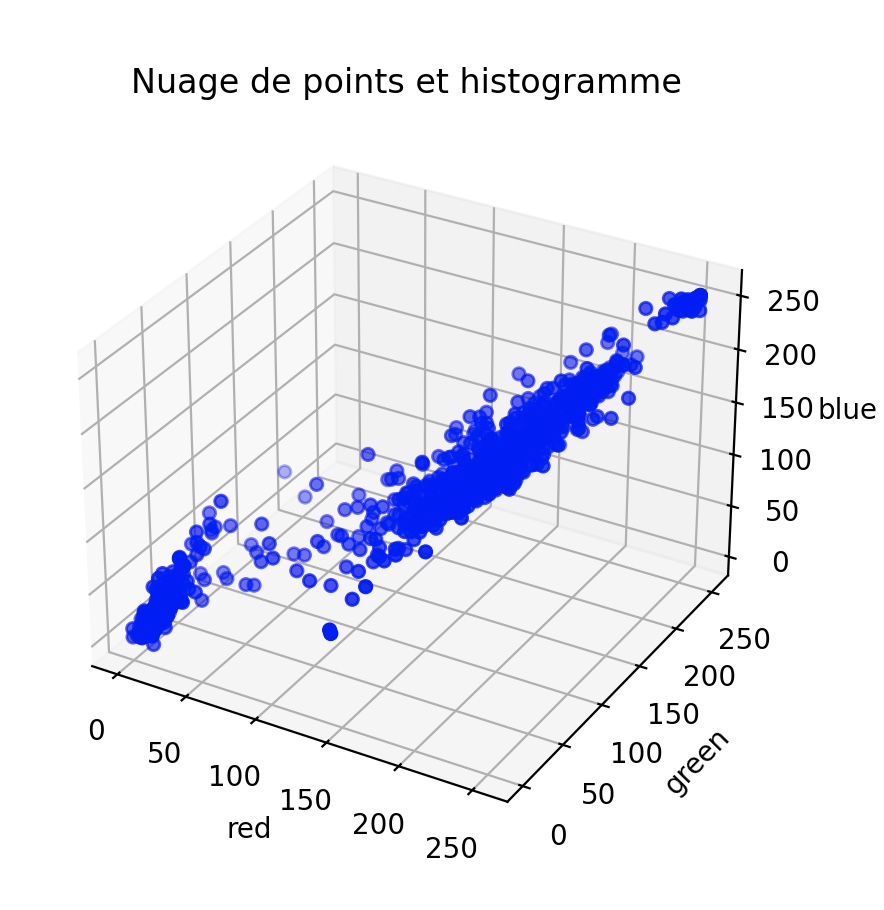
\includegraphics[width=0.75\textwidth]{./img/5.1.1.jpg}
            \caption{\label{fig:1.2}Image 3D}  
        \end{center}
    \end{minipage}
\end{figure}

\clearpage 

\textbf{Question 2: Descriptions des graphiques} \\

Sur le premier graphique 2D, on distingue 9 sous-graphiques combinaison des trois couleurs RGB. Ce qui se retrouve sur
chacun des sous-graphiques c'est la distinction de trois clusters. En effet, on a trois niveaux d'intensités différents,
un très bas, ce qui correspond à la couleur la plus foncée, la mer, un moyen, ce qui correspond à la couleur de la terre
sur les extérieurs de l'image et un haut, ce qui correspondant à la terre qui fait le contour de la mer. \\

Sur le deuxième graphique 3D, on peut faire la même analyse mais cette fois-ci, on peut dire que l'on regroupe tous les
sous-graphiques précédents, ce qui nous permet de disintguer clairement chacun des clusters. Les clusters sont donc la mer, 
la terre et le rivage. 








